\documentclass{standalone}
\usepackage{tikz}
\usepackage{pgfplots}
\usetikzlibrary{arrows, decorations.pathmorphing}

\pgfplotsset{compat = 1.15}


\pgfmathdeclarefunction{gauss}{3}{%
  \pgfmathparse{1/(#3*sqrt(2*pi))*exp(-((#1-#2)^2)/(2*#3^2))}%
}

\begin{document}

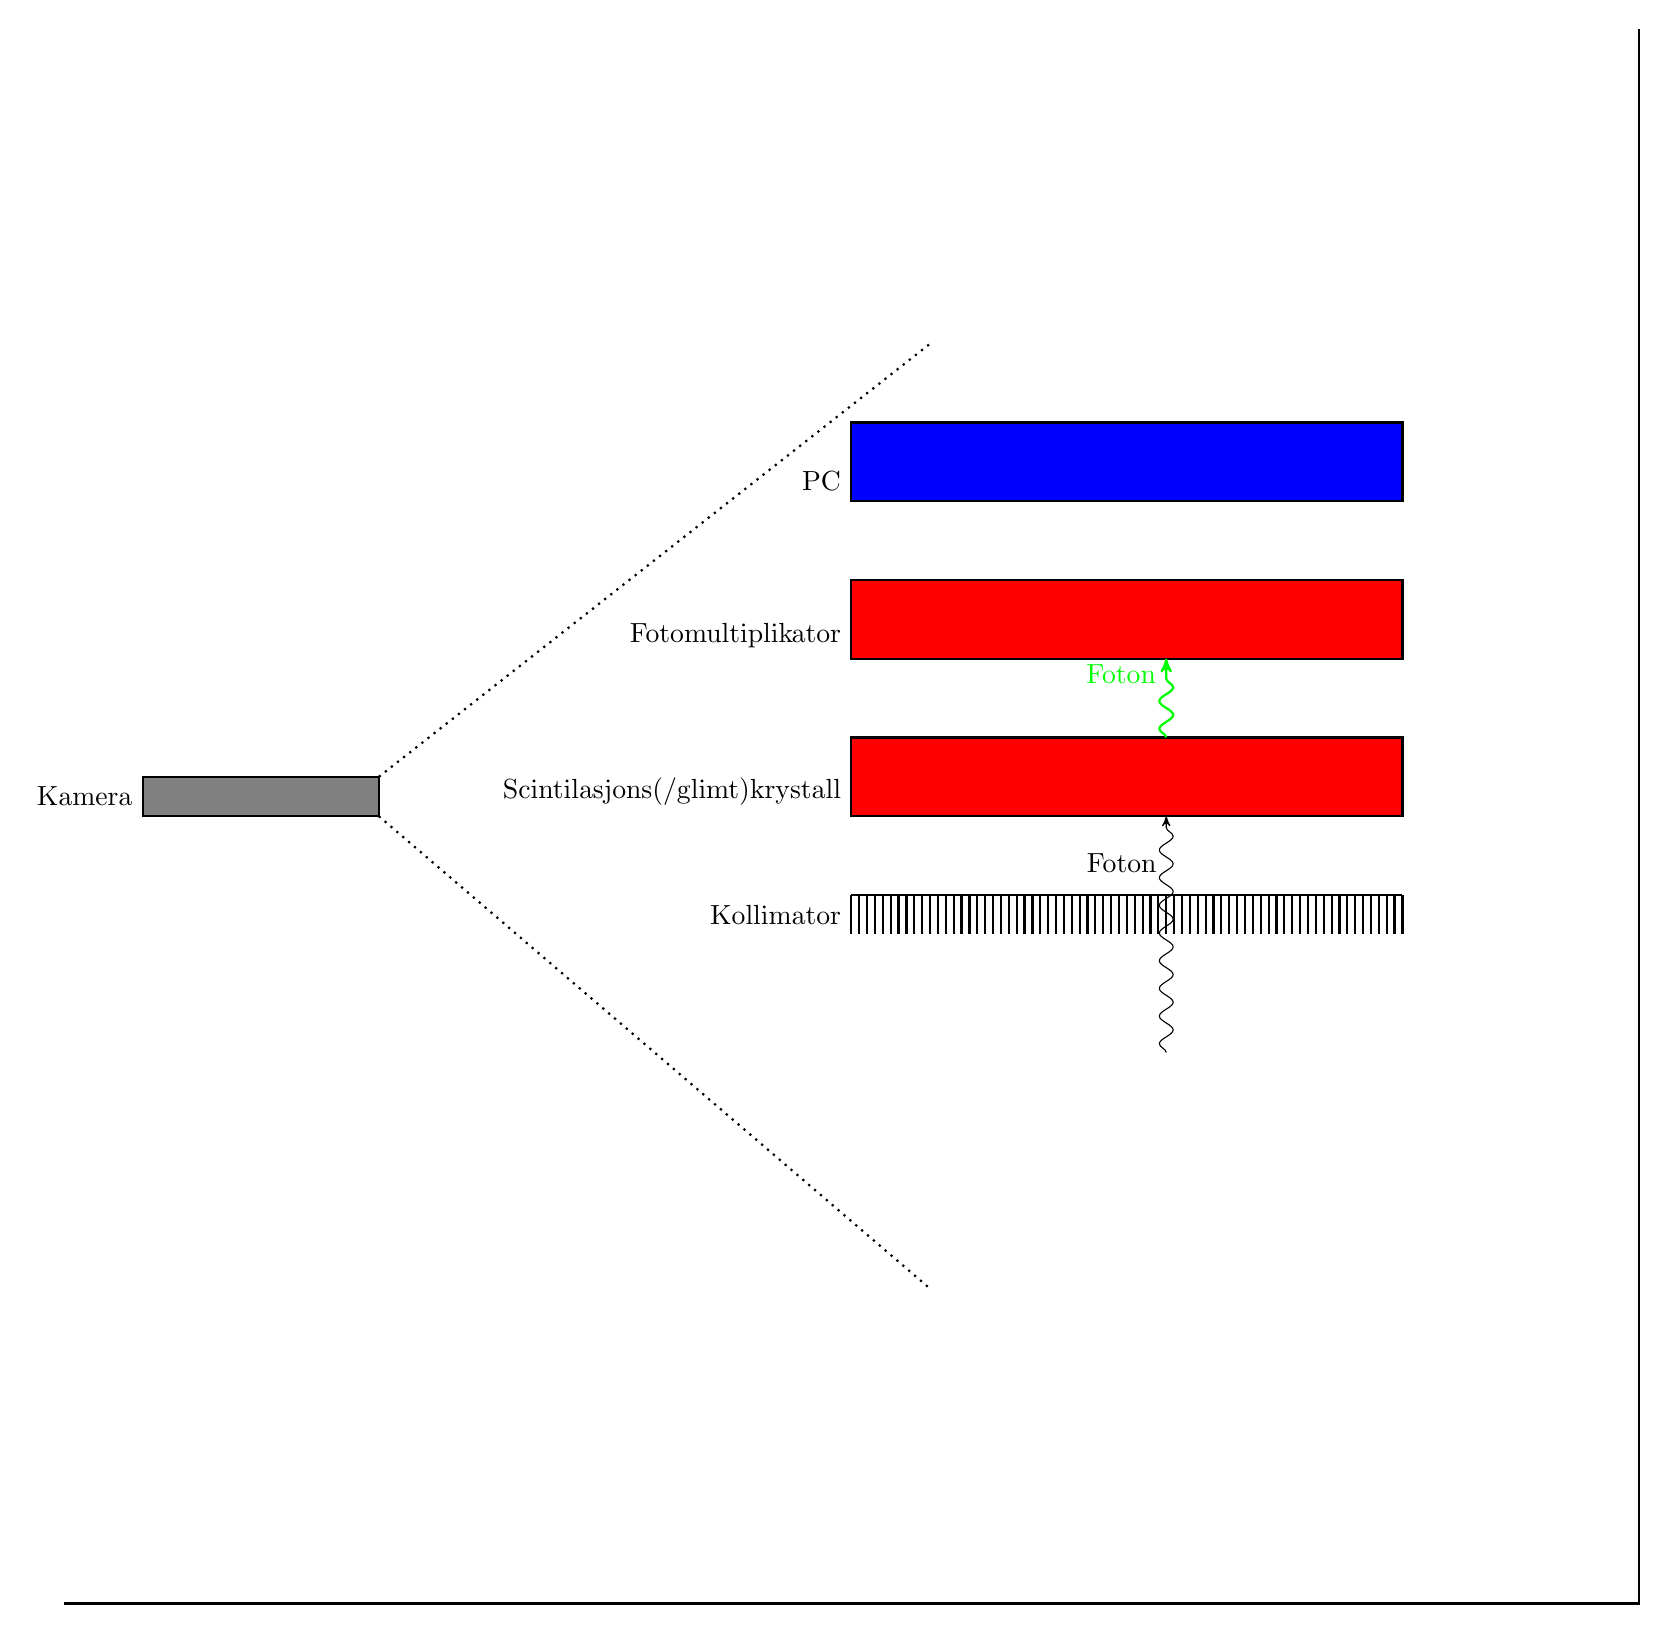
\begin{tikzpicture}[
    >=stealth',
    pos = .8,
    photon/.style = {decorate, decoration = {snake, post length=1mm}}]

\draw[thick] (-10, -10) -- (10, -10) -- (10, 10);

\draw[thick, fill=gray] (-9, 0) node [above left] {Kamera} rectangle (-6,0.5); % The camera

\draw[thick, style = dotted] (-6,0.5) -- (1,6);
\draw[thick, style = dotted] (-6,0) -- (1,-6);



\draw[thick, fill=red] (0, 0) node [above left] {Scintilasjons(/glimt)krystall} rectangle (7,1) ;


\draw[thick, fill=red] (0, 2) node [above left] {Fotomultiplikator} rectangle (7,3);

\draw[thick, fill=blue] (0, 4) node [above left] {PC} rectangle (7,5);

\draw[thick] (0, -1) node [below left] {Kollimator}  -- (7, -1);

\draw[thick] (0.0, -1) -- (0.0, -1.5);
\draw[thick] (0.1, -1) -- (0.1, -1.5);
\draw[thick] (0.2, -1) -- (0.2, -1.5);
\draw[thick] (0.3, -1) -- (0.3, -1.5);
\draw[thick] (0.4, -1) -- (0.4, -1.5);
\draw[thick] (0.5, -1) -- (0.5, -1.5);
\draw[thick] (0.6, -1) -- (0.6, -1.5);
\draw[thick] (0.7, -1) -- (0.7, -1.5);
\draw[thick] (0.8, -1) -- (0.8, -1.5);
\draw[thick] (0.9, -1) -- (0.9, -1.5);
\draw[thick] (1.0, -1) -- (1.0, -1.5);
\draw[thick] (1.1, -1) -- (1.1, -1.5);
\draw[thick] (1.2, -1) -- (1.2, -1.5);
\draw[thick] (1.3, -1) -- (1.3, -1.5);
\draw[thick] (1.4, -1) -- (1.4, -1.5);
\draw[thick] (1.5, -1) -- (1.5, -1.5);
\draw[thick] (1.6, -1) -- (1.6, -1.5);
\draw[thick] (1.7, -1) -- (1.7, -1.5);
\draw[thick] (1.8, -1) -- (1.8, -1.5);
\draw[thick] (1.9, -1) -- (1.9, -1.5);
\draw[thick] (2.0, -1) -- (2.0, -1.5);
\draw[thick] (2.1, -1) -- (2.1, -1.5);
\draw[thick] (2.2, -1) -- (2.2, -1.5);
\draw[thick] (2.3, -1) -- (2.3, -1.5);
\draw[thick] (2.4, -1) -- (2.4, -1.5);
\draw[thick] (2.5, -1) -- (2.5, -1.5);
\draw[thick] (2.6, -1) -- (2.6, -1.5);
\draw[thick] (2.7, -1) -- (2.7, -1.5);
\draw[thick] (2.8, -1) -- (2.8, -1.5);
\draw[thick] (2.9, -1) -- (2.9, -1.5);
\draw[thick] (3.0, -1) -- (3.0, -1.5);
\draw[thick] (3.1, -1) -- (3.1, -1.5);
\draw[thick] (3.2, -1) -- (3.2, -1.5);
\draw[thick] (3.3, -1) -- (3.3, -1.5);
\draw[thick] (3.4, -1) -- (3.4, -1.5);
\draw[thick] (3.5, -1) -- (3.5, -1.5);
\draw[thick] (3.6, -1) -- (3.6, -1.5);
\draw[thick] (3.7, -1) -- (3.7, -1.5);
\draw[thick] (3.8, -1) -- (3.8, -1.5);
\draw[thick] (3.9, -1) -- (3.9, -1.5);
\draw[thick] (4.0, -1) -- (4.0, -1.5);
\draw[thick] (4.1, -1) -- (4.1, -1.5);
\draw[thick] (4.2, -1) -- (4.2, -1.5);
\draw[thick] (4.3, -1) -- (4.3, -1.5);
\draw[thick] (4.4, -1) -- (4.4, -1.5);
\draw[thick] (4.5, -1) -- (4.5, -1.5);
\draw[thick] (4.6, -1) -- (4.6, -1.5);
\draw[thick] (4.7, -1) -- (4.7, -1.5);
\draw[thick] (4.8, -1) -- (4.8, -1.5);
\draw[thick] (4.9, -1) -- (4.9, -1.5);
\draw[thick] (5.0, -1) -- (5.0, -1.5);
\draw[thick] (5.1, -1) -- (5.1, -1.5);
\draw[thick] (5.2, -1) -- (5.2, -1.5);
\draw[thick] (5.3, -1) -- (5.3, -1.5);
\draw[thick] (5.4, -1) -- (5.4, -1.5);
\draw[thick] (5.5, -1) -- (5.5, -1.5);
\draw[thick] (5.6, -1) -- (5.6, -1.5);
\draw[thick] (5.7, -1) -- (5.7, -1.5);
\draw[thick] (5.8, -1) -- (5.8, -1.5);
\draw[thick] (5.9, -1) -- (5.9, -1.5);
\draw[thick] (6.0, -1) -- (6.0, -1.5);
\draw[thick] (6.1, -1) -- (6.1, -1.5);
\draw[thick] (6.2, -1) -- (6.2, -1.5);
\draw[thick] (6.3, -1) -- (6.3, -1.5);
\draw[thick] (6.4, -1) -- (6.4, -1.5);
\draw[thick] (6.5, -1) -- (6.5, -1.5);
\draw[thick] (6.6, -1) -- (6.6, -1.5);
\draw[thick] (6.7, -1) -- (6.7, -1.5);
\draw[thick] (6.8, -1) -- (6.8, -1.5);
\draw[thick] (6.9, -1) -- (6.9, -1.5);
\draw[thick] (7.0, -1) -- (7.0, -1.5);

% Signals 

\begin{scope}[xshift = 4cm, yshift = -3cm,  rotate around= {90:(0,0)}]
\draw[->, photon] (0,0) -- node [left] {Foton} (0:3);
\end{scope}

\begin{scope}[xshift = 4cm, yshift = 1cm,  rotate around= {90:(0,0)}]
\draw[->, photon, thick, green] (0,0) -- node [left] {Foton} (0:1);
\end{scope}





\end{tikzpicture}

\end{document}